\subsection{Flächentreue Albert-Projektion}
\label{sec:albert}
Die flächentreue Albert-Projektion ist eine globale Kegelprojektion. Sie bildet die Erde auf einen Kegelmantel ab. Sie benutzt für die Projektion 2 Standardbreitenkreise. 
\\

Formel:\\ 
\begin{eqnarray*}
\mathcal{X}&=&\rho \sin \theta \\
\mathcal{Y}&=&\rho _0 -\rho \cos \theta\\
\\
n&=&\frac{1}{2}(\sin \varphi _1 +\sin \varphi _2)\\
\theta &=&n(\lambda -\lambda _0)\\
\tau &=&\cos ^2 \varphi _1 +2n\sin \varphi _1\\
\rho &=&\dfrac{\sqrt{\tau -2n\sin \varphi}}{n}\\
\rho _0 &=&\dfrac{\sqrt{\tau -2n\sin \varphi _0}}{n}
\end{eqnarray*}

\begin{figure}[hbtp]
\centering
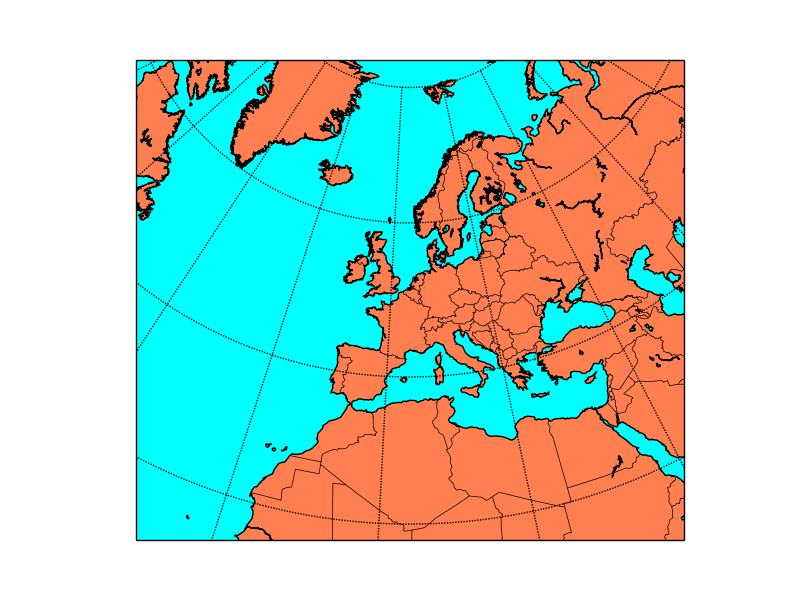
\includegraphics[scale=0.5,origin=c]{/Users/student/seminar/Kartendarstellungen/seminar/aea} \\
\caption{Flächentreue Albert-Projektion}
\end{figure}
\newpage 